

\documentclass{article}
\usepackage[utf8]{inputenc}
\usepackage[english]{babel}
\usepackage[]{amsthm} %lets us use \begin{proof}
\usepackage[]{amssymb} %gives us the character \varnothing
\usepackage{graphicx}
\usepackage{hyperref}
\usepackage{multicol}


\title{Homework 3}
\author{Aasim Zahoor}
\date\today


\begin{document}
\maketitle 


\begin{center}
\section{Problems}
\end{center}
\textbf{Link}\vspace{1.5em}
\url{https://github.com/AasimZahoor/Comp_methods.git}
\vspace{1.5em}

\textbf{Problem 1}\vspace{1.5em}
\\
In this problem I use two random matrices to test my matrix class. I used numpy's functionality to test some of the instances of the class. There were 7 instances in my class and I tested all of them. So I tested addition, multiplication, transpose, trace, Determinant, Inverse and LU decomposition. The output is:
\\*
\\*
\begin{center}
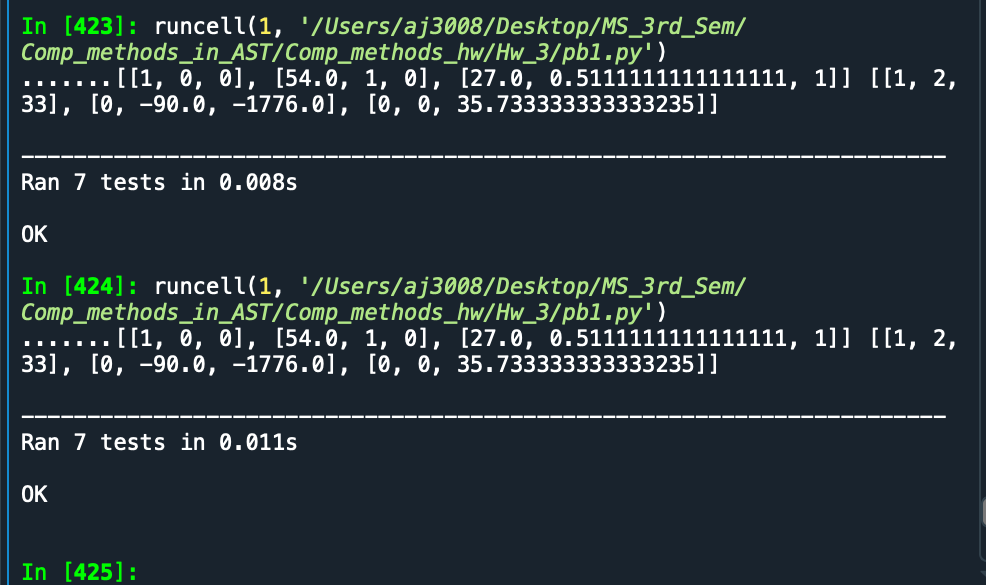
\includegraphics[scale=0.5]{/Users/aj3008/Desktop/MS_3rd_Sem/Comp_methods_in_AST/Comp_methods/Hw_3/Latex/Images/pb1}
\end{center}

\clearpage





\textbf{Problem 2}\vspace{1.5em}

This problem asks us to plot number densities at different temperatures. I took 8 temperature values. They are $T=[273,1000,4000,8000,10000,30000,50000,60000]$. For this problem I first found the pattern and wrote an algorithm for it. Here is a test for 3 state system. Note the coefficients are such that the RHS of equation formed is zero, meaning I took the LHS in the equations(on the Homework sheet) you gave to RHS.

\begin{center}
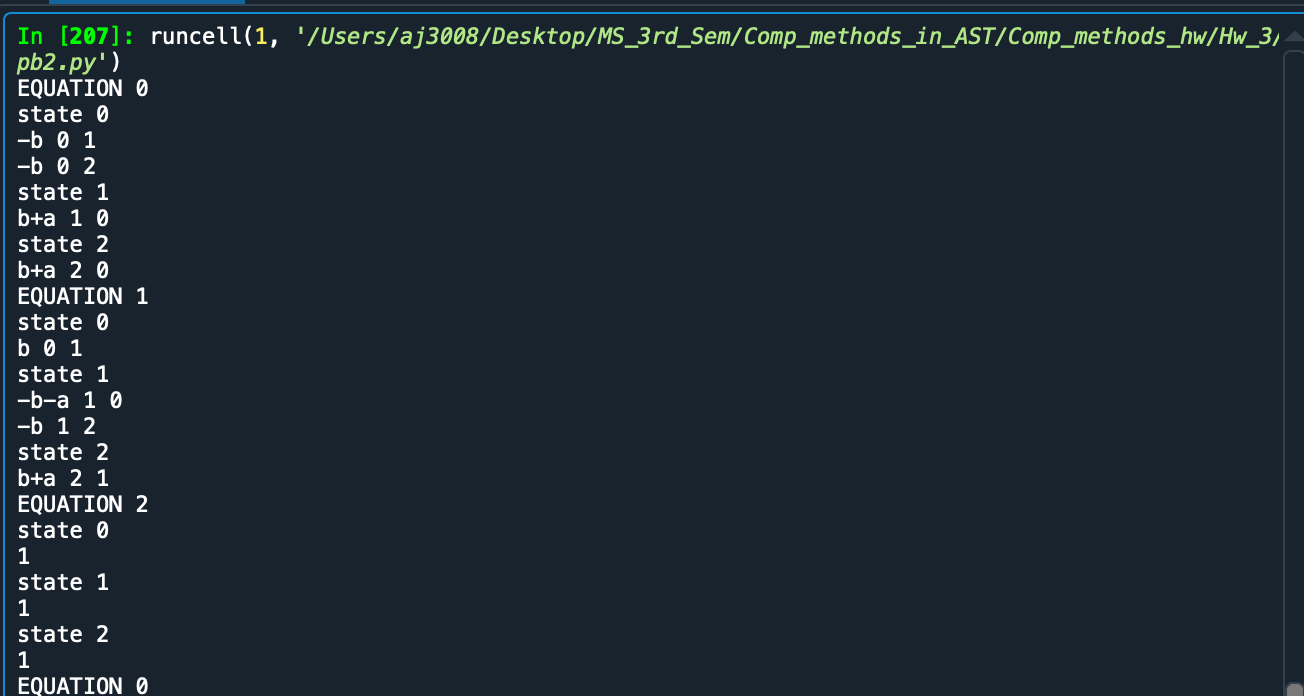
\includegraphics[scale=0.5]{/Users/aj3008/Desktop/MS_3rd_Sem/Comp_methods_in_AST/Comp_methods/Hw_3/Latex/Images/Pattern}
\\*
\textbf{Figure}: Testing the alogorithm
\end{center}

After finding the pattern I wrote down functions for Bul, Aul, Blu and Energy. Then I extracted the data and plotted the number densities V/s Temperature.
\begin{center}
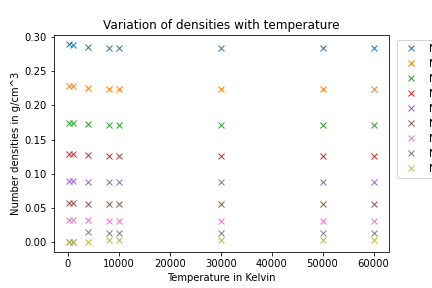
\includegraphics[scale=0.9]{/Users/aj3008/Desktop/MS_3rd_Sem/Comp_methods_in_AST/Comp_methods/Hw_3/Latex/Images/pb2}
\\*
\textbf{Figure}: Plot of number densities v/s temperature
\end{center} 
The number density decreases for lower states and increases for higher states as temperature is increased. It makes sense as we increase temperature, electron will have more energy available to them, allowing them to spend more time in higher states.


\clearpage
\textbf{Problem 3}\vspace{1.5em}
\\
In the code for Problem 3 I have defined 3 functions. They are:
\begin{itemize}
\item{\textbf{euler$(x_0,y_0,f,h,k)$}}
This function call euler method for solving ODE. The arguments are:
\\*
       $ x_0$=initial x value
        $y_0$=initial y value
        $f$=function of x,y,t
        h=step size
        k=number of times
       \\*
        It returns x,y,t values in that order


\item{\textbf{heun$(x_0,y_0,f,h,k,p=10)$}}\vspace{0.2em}

This function call Heun's method for solving ODE. The arguments are:
\\*
        $x_0$=initial x value, 
        $y_0$=initial y value, 
        $f$=function of x,y,t, 
        h=step size, 
        k=number of times, 
        p=picard's iteration (Default value 10)
        \\*
        It returns x,y,t values in that order


\item{\textbf{rk$(x_0,y_0,f,h,k)$}}\vspace{0.2em}

This function call RK-4 method for solving ODE. The arguments are:
\\*
      $ x_0$=initial x value, 
        $y_0$=initial y value, 
        $f$=function of x,y,t, 
        h=step size, 
        k=number of times
        \\*
        It returns x,y,t values in that order


\vspace{0.2em}

\end{itemize}

\vspace{1.5em}
\textbf{Problem 4}\vspace{1.5em}
\\
In this problem we are supposed to test the functions we wrote in problem 3 using the pendulum function. To model the function I have made a function called \textbf{f(b,c)}. This function takes two arguments, b= coefficient of y, c= coefficient of g(x,t). This function returns an array where the first element gives d(theta)/dt and the second element returns d(omega)/dt. They values of b is taken to be 0.25 and c is 5, step size is 0.1 and k (number of times) is 50 (to see the difference between the three methods) and 200 (to see how damping works).
\\



 \begin{center}
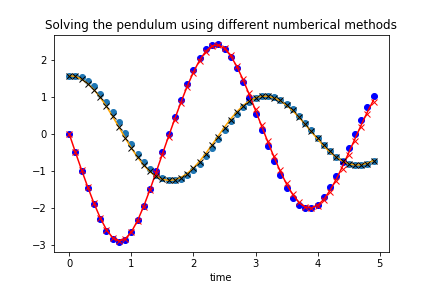
\includegraphics[scale=0.35]{/Users/aj3008/Desktop/MS_3rd_Sem/Comp_methods_in_AST/Comp_methods/Hw_3/Latex/Images/pb4}
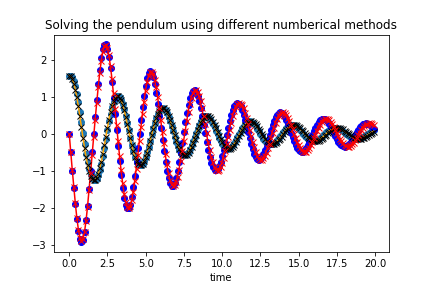
\includegraphics[scale=0.35]{/Users/aj3008/Desktop/MS_3rd_Sem/Comp_methods_in_AST/Comp_methods/Hw_3/Latex/Images/pb4_1}

\textbf{Figure}: The figure on the left is for k=50 and one on the right is for k=200
\end{center}

\vspace{0.2em}

\clearpage
\textbf{Problem 5}\vspace{1.5em}
\\
In this problem we are supposed to test our methods on the given equation. I defined a function \textbf{f(l)} which returns the function given in pb5. It takes lambda as input and gives an array as output where first element is always 1 and second element gives dy/dt in terms of y and t. The reason it gives 1 as the first element is because my ODE solvers were made for 2 dependent variables and this has only 1. All three methods seem stable for this equation. The difference between analytical solution and solution provided by each method don't seem to be differentmuch. However, Euler's method is a bit off in the beginning where we can say it is less stable.


 \begin{center}
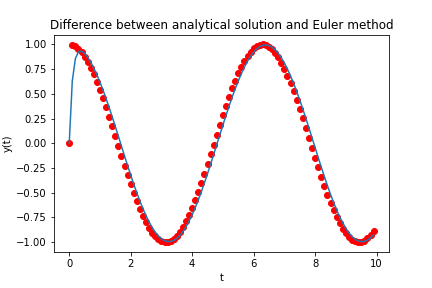
\includegraphics[scale=0.35]{/Users/aj3008/Desktop/MS_3rd_Sem/Comp_methods_in_AST/Comp_methods/Hw_3/Latex/Images/pb5_e}
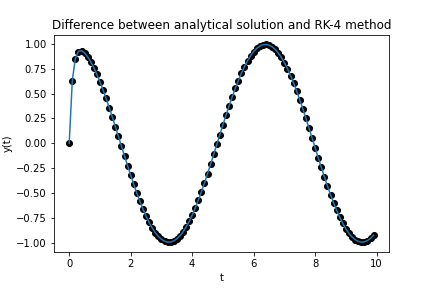
\includegraphics[scale=0.35]{/Users/aj3008/Desktop/MS_3rd_Sem/Comp_methods_in_AST/Comp_methods/Hw_3/Latex/Images/pb5_r}
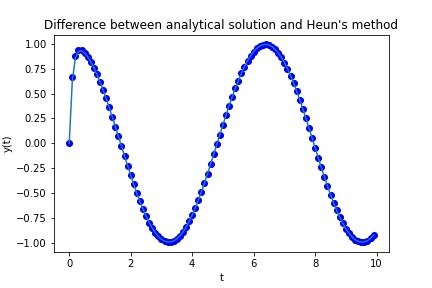
\includegraphics[scale=0.35]{/Users/aj3008/Desktop/MS_3rd_Sem/Comp_methods_in_AST/Comp_methods/Hw_3/Latex/Images/pb5_h}

\textbf{Figure}: These figures shows the three methods against the analytical solution.
\end{center}


        
     














\end{center}

\vspace{0.2em}
\end{document}
